\documentclass{article}
\usepackage[utf8]{inputenc}
\usepackage{hyperref}
\documentclass{article}
\usepackage{listings}
\usepackage{amsmath}
\usepackage{subfig}
\usepackage{amsthm}
\usepackage{amsmath}
\usepackage{amssymb}
\usepackage{graphicx}
\usepackage{mdwlist}
\usepackage{geometry}
\usepackage{titlesec}
\usepackage{palatino}
\usepackage{mathrsfs}
\usepackage{fancyhdr}
\usepackage{paralist}
\usepackage{todonotes}
\usepackage{tikz}
\usepackage{float} % Place figures where you ACTUALLY want it
\usepackage{comment} % A hack to toggle sections
\usepackage{ifthen}
\usepackage{mdframed}
\usepackage{verbatim}
\usepackage{listings}
\usepackage{bbm}
\usepackage{upquote} % Prevents backticks replacing single-quotes in verbatim
\usepackage[strings]{underscore}
\usepackage[colorlinks=true]{hyperref}
\usetikzlibrary{positioning,shapes,backgrounds}

\geometry{margin=1in}
\geometry{headheight=2in}
\geometry{top=2in}

\setlength{\marginparwidth}{2.15cm}
\setlength{\parindent}{0em}
\setlength{\parskip}{0.6\baselineskip}

\rhead{}
\lhead{}

% Spacing settings.
\titlespacing\section{0pt}{12pt plus 2pt minus 2pt}{0pt plus 2pt minus 2pt}
\titlespacing\subsection{0pt}{12pt plus 4pt minus 2pt}{0pt plus 2pt minus 2pt}
\titlespacing\subsubsection{0pt}{12pt plus 4pt minus 2pt}{0pt plus 2pt minus 2pt}
\renewcommand{\baselinestretch}{1.15}

% Shortcuts for commonly used operators.
\newcommand{\E}{\mathbb{E}}
\newcommand{\Var}{\operatorname{Var}}
\newcommand{\Cov}{\operatorname{Cov}}
\newcommand{\Bias}{\operatorname{Bias}}
\DeclareMathOperator{\argmin}{arg\,min}
\DeclareMathOperator{\argmax}{arg\,max}

% Do not number subsections and below.
\setcounter{secnumdepth}{1}

% Custom format subsection.
\titleformat*{\subsection}{\large\bfseries}

% Set up the problem environment.
\newcounter{problem}[section]
\newenvironment{problem}[1][]
  {\begingroup
    \setlength{\parskip}{0em}
    \refstepcounter{problem}\par\addvspace{1em}\textbf{Problem~\Alph{problem}\!
    \ifthenelse{\equal{#1}{}}{}{ [#1 points]}:}
  \endgroup}

% Set up the subproblem environment.
\newcounter{subproblem}[problem]
\newenvironment{subproblem}[1][]
  {\begingroup
    \setlength{\parskip}{0em}
    \refstepcounter{subproblem}\par\medskip\textbf{\roman{subproblem}.\!
    \ifthenelse{\equal{#1}{}}{}{ [#1 points]:}}
  \endgroup}

% Set up the teachers and materials commands.
\newcommand\teachers[1]
  {\begingroup
    \setlength{\parskip}{0em}
    \vspace{0.3em} \textit{\hspace*{2em} TAs responsible: #1} \par
  \endgroup}
\newcommand\materials[1]
  {\begingroup
    \setlength{\parskip}{0em}
    \textit{\hspace*{2em} Relevant materials: #1} \par \vspace{1em}
  \endgroup}

% Set up the hint environment.
\newenvironment{hint}[1][]
  {\begin{em}\textbf{Hint: }}
  {\end{em}}


% Set up the solution environment.
\ifshowsolutions
  \newenvironment{solution}[1][]
    {\par\medskip \begin{mdframed}\textbf{Solution~\Alph{problem}#1:} \begin{em}}
    {\end{em}\medskip\end{mdframed}\medskip}
  \newenvironment{subsolution}[1][]
    {\par\medskip \begin{mdframed}\textbf{Solution~\Alph{problem}#1.\roman{subproblem}:} \begin{em}}
    {\end{em}\medskip\end{mdframed}\medskip}
\else
  \excludecomment{solution}
  \excludecomment{subsolution}
\fi

\title{CS 155 Group Project 2 Report}
\author{Joon Young Park, Derek Ing, Daniel Li, Hernan Caceres}
\date{February 2022}

\begin{document}

\maketitle

\section{Introduction}

\begin{enumerate}
    \item \textbf{Group members}:
    \vspace{2mm} 
    
    Hernan Caceres, Daniel Li, Derek Ing, Joon Young Park
    
    \item \textbf{Colab Link}:
    \vspace{1.5mm} 
    
    \href{https://colab.research.google.com/drive/1R8D9uk7o5qWmJ62WFXMZSglOFGF19Hun?usp=sharing}{ 
Click here.}
    
    \item \textbf{Piazza Link}:
    \vspace{1.5mm} 
    
    \href{https://piazza.com/class/kxhtyed0nmh2s?cid=392}{ 
Click here.} 
    
    \item \textbf{Division of Labor}:
    \vspace{1.5mm} 
    
    \begin{enumerate}

        \item Derek Ing: Matrix Factorization 2
        
        \item Daniel Li: Matrix Factorization 1
        
        \item Joon Young Park: Basic Visualizations and GridSearch for parameters
        
        \item Hernan Caceres: Matrix Factorization 3
    \end{enumerate}
\end{enumerate}

\newpage

\section{Basic Visualizations}

\subsection{All ratings in the MovieLens Dataset}

\begin{figure}[H] \begin{center}
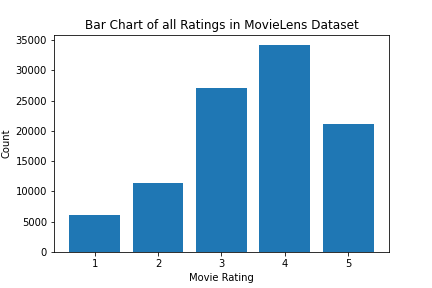
\includegraphics[width=0.7\textwidth]{basicvisualizations/Bar Chart of All Ratings.png}
\end{center} \end{figure}

\subsection{All ratings of the ten most popular movies}

\begin{figure}[H] \begin{center}
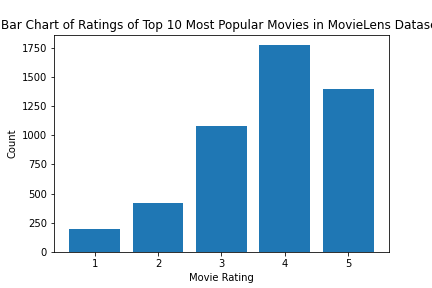
\includegraphics[width=0.7\textwidth]{basicvisualizations/Bar Chart of Top 10 Most Popular Movies Ratings.png}
\end{center} \end{figure}

\subsection{All ratings of the ten best movies}

\begin{figure}[H] \begin{center}
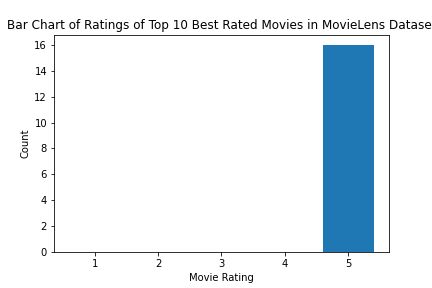
\includegraphics[width=0.7\textwidth]{basicvisualizations/Bar Chart of Top 10 Best Rated Movies Ratings.png}
\end{center} \end{figure}

\subsection{All ratings of movies from three genres of your choice}

\begin{figure}[H] \begin{center}
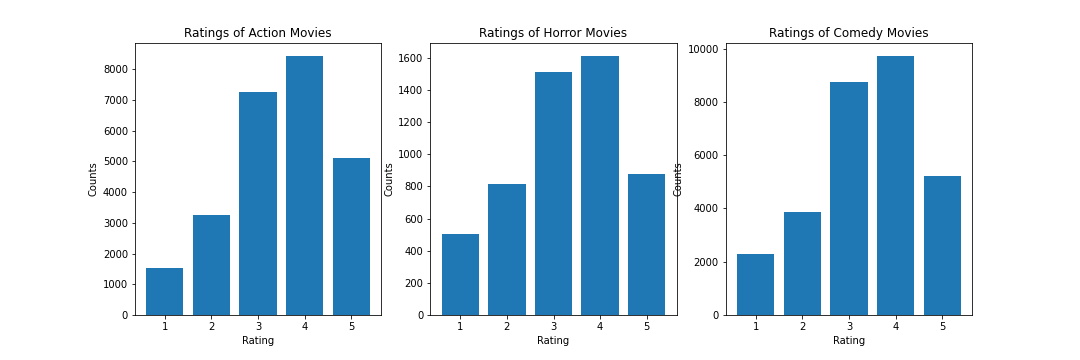
\includegraphics[width=\textwidth]{basicvisualizations/Bar Charts of Ratings by Genre.png}
\end{center} \end{figure}

In general, we observed that the distribution of movie ratings is skewed left and the most frequent rating given is 4. The results also did match what we expected to see. From our experience, we do not usually watch movies that are rated very bad online or we do not think we would enjoy, which could be the case for the users in the dataset, too. If we tend to watch movies that we think we would like, then we would also rate these movies well. If we happen to watch a movie that we strongly dislike, then we would rate it badly. \\
Comparing the ten best movies and the ten most popular movies, all of ten best movies only have ratings of 5. In addition, there are not many ratings for the ten best movies. From the best rated movies histogram, there are a total of 16 ratings for the 10 best movies. The 10 most popular movies has a ratings distribution similar to the ratings of all movies in the dataset. This makes sense because these are the most rated movies, so it is likely the ratings distribution of the most popular movies is similar to that of all movies. \\
We chose action, horror, and comedy as our three genres. All of the three genres have similar ratings distributions, with 4 being the most frequent rating and they are all left skewed. Horror movies, however, has a high proportion of 3 ratings compared to the other genres. This could be attributed to the fact that a lot of people would get very scared watching a horror movie and dislike that feeling. 

\newpage


\section{Matrix Factorization Methods}
For method 1, we use collaborative filtering to construct two matrices, $U \in \mathbb{M}_{k x m}$ and $V \in \mathbb{M}_{k x n}$, to represent a matrix $Y \in \mathbb{M}_{m x n} \cong U^TV$. The matrix $Y$ represents each user's ratings for each movie in the dataset, where $m = 943$ is the number of users, $n = 1682$ is the number of movies, and $k=20$ is the number of latent factors. The element $Y_{ij}$ represents user $i$'s rating for movie $j$. In the given data set, users do not rate all the movies, thus we have unknown rating values. Thus, we use collaborative filtering to a learn latent representation of movies $U$ and users $V$ to explain the observed ratings, and thus predict all users ratings of all the movies.
We learn a latent representation such that $$\argmin_{U,V} \frac{\lambda}{2} \left( \|U\|_F^2 + \|V\|^2_F \right) + \frac{1}{2}\sum_{i,j} \left( y_{ij} - u_{i}^Tv_j\right)^2$$ where $u^i$ and $v^j$ are the $i$th and $j$th columns of U and V, respectively. We first initialize U and V matrices by randomly drawing samples from a uniform distribution between $(-0.5,0.5)$. Then, for each epoch, randomly iterate through each data point, $(i, j, y_{ij})$, in the training set and update $u_i$ and $v_j$ by stochastic gradient descent. We calculate gradients 
$$\delta{u_i} = \lambda u_i - v_j(y_{ij} - u_i^Tv_j)$$
$$\delta{v_j} = \lambda v_j - u_i(y_{ij} - u_i^Tv_j)$$ and update $u_i = u_i - \eta \delta{u_i}$ and $v_j = v_j - \eta \delta{v_j}$ accordingly, where we chose our learning rate, $\eta$. We implement an early stopping condition and stop at epoch $t$ if $\Delta_{t-1,t} / \Delta_{0,1} \leq \epsilon = 0.0001$, where $\Delta_{t-1,t}$ is the loss reduction between epoch $t$ and $t-1$ and $\Delta_{0,1}$ is the loss reduction between before training and after the first epoch.

For methods 2 and 3, we used the Surprise package's SVD algorithm. In method 3, we set the bias parameter to False so that there are no bias terms, and in method 2 we include bias terms. The Surprise SVD algorithm learns $U \in \mathbb{M}_{m x k}$ and $V \in \mathbb{M}_{n x k}$, to represent a matrix $Y \in \mathbb{M}_{m x n} \cong UV^T$. \\

For method 2, all biases are initialized to 0 and U and V are randomly initialized by drawing from a normal distribution with $\mu = 0$ and $\sigma = 1$. The predictions are set to $\hat{r} = \mu + b_i + b_j + u_i^{T}v_j$.\\ The algorithm also minimizes $$\sum_{r_{ij} \in R_{train}} (r_{ij} - \hat{r}_{ij})^2 + \lambda (b_i^2 + b_j^2 + ||u_i||^2 + ||v_j||^2)$$ 
Surprise's implementation also uses stochastic gradient descent to update $u_i$, $v_j$, and the bias terms, $b_i$ and $b_j$. The updates are performed by $$b_i = b_i + \gamma(e_{ij} - \lambda b_i)$$
$$b_j = b_j + \gamma(e_{ij} - \lambda b_j)$$
$$u_i = u_i + \gamma(e_{ij} v_j - \lambda u_i)$$
$$v_j = v_j + \gamma(e_{ij} u_i - \lambda v_j)$$
where $e_{ij} = r_{ij} - \hat{r_{ij}}$ and $\gamma$ is the learning rate. The updates are performed for $n$ epochs and there is no early stopping condition. This is the same for method 3 except biases are not included in the learning objective and are not updated. \\

For method 1, we trained for different values of $\lambda$ and $\eta$ to find the parameters that minimize unregularized mean squared error on the test set. For methods 2 and 3, we performed a grid search for different values of $\lambda$ and $\gamma$ to minimize root mean squared error.\\

Loss curves for method 1 matrix factorization, the x axis represents values of $\eta$:\\
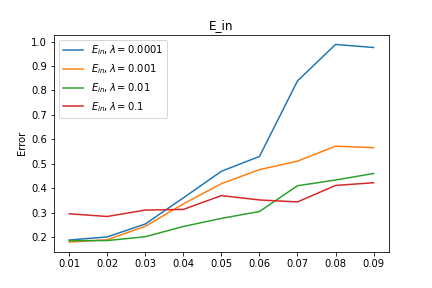
\includegraphics[width=0.5\textwidth]{E_in vs Error.png}
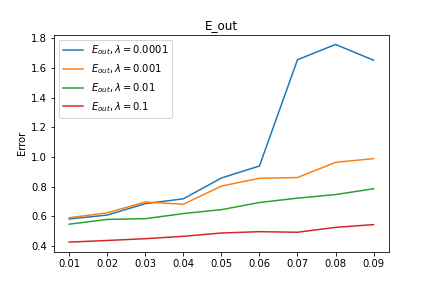
\includegraphics[width=0.5\textwidth]{E_out vs Error.png}\\
After training, our errors on the test set were: method 1 = $0.429$, method 2 = $1.329$, and method 3 = $1.430$. Method 2 is different from methods 1 and 3 because it includes bias terms. Methods 2 and 3 also do not use an early stopping condition while method 1 does. Method 1 is different from methods 2 and 3 because we initialize $U$ and $V$ according to a uniform distribution as opposed to initializing according to a normal distribution. \\
The early stopping condition could attribute to method 1 performing better than method 2. With early stopping, we prevent the model from overfitting to the training set. Without early stopping, the model can overfit to the training set, and thus cannot generalize and perform well on the test set. \\

Between methods 2 and 3, the model with the bias term performs slightly better than the model without the bias term. Some movies are rated higher/lower on average compared to other movies. On the other hand, some users may give on average higher/lower ratings to movies compared to other users. Thus, to compare a user's ratings to other users, we do not want to take into account the bias of a user. The bias term can help us remove this user bias. In addition, when we make predictions for a user's rating of a certain movie, we can also take into account a certain user's rating tendencies. As a result, the bias terms can help the model better capture the interactions between the users and movies, and thus the model can perform better than without bias terms.

\newpage

\section{Matrix Factorization Visualizations}

\subsection{10 Movies of Our Choice}

\begin{figure}[H]
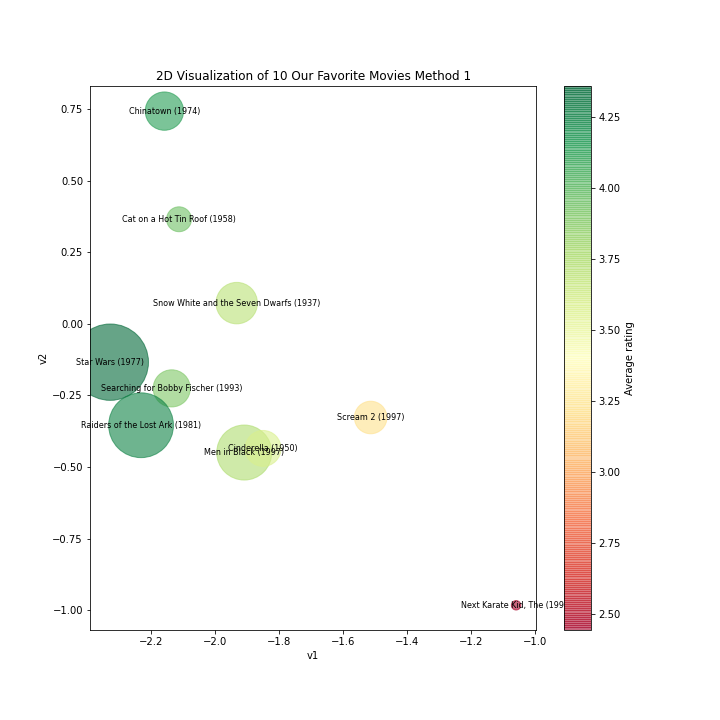
\includegraphics[width=0.5\textwidth]{matrixfactorization/2D Visualization of 10 Our Favorite Movies Method 1.png}
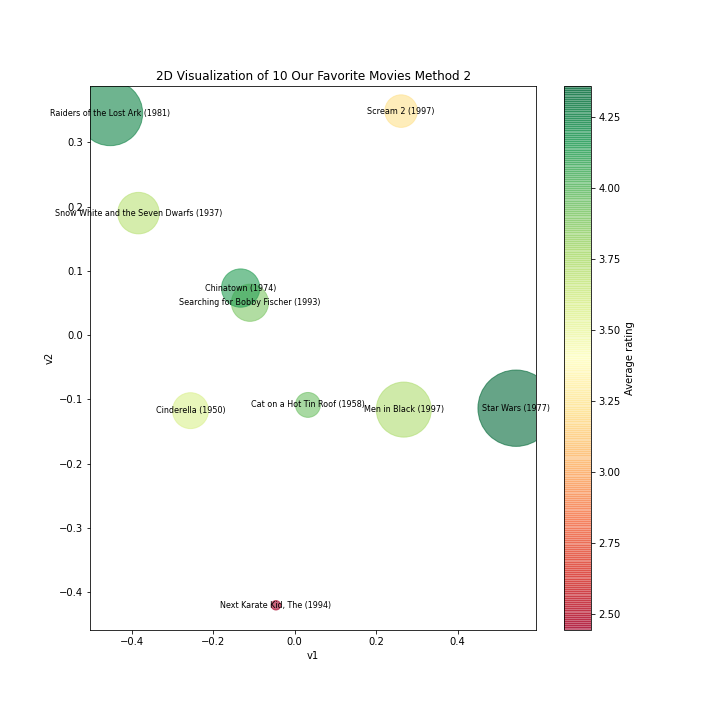
\includegraphics[width=0.5\textwidth]{matrixfactorization/2D Visualization of 10 Our Favorite Movies Method 2.png}
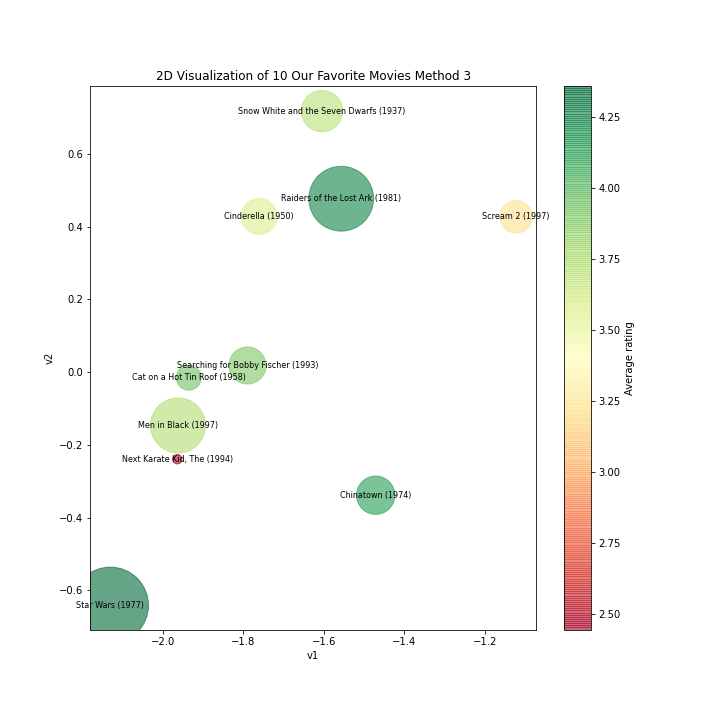
\includegraphics[width=0.5\textwidth]{matrixfactorization/2D Visualization of 10 Our Favorite Movies Method 3.png}
\end{figure}

\newpage

\subsection{10 Most Popular Movies}

\begin{figure}[H]
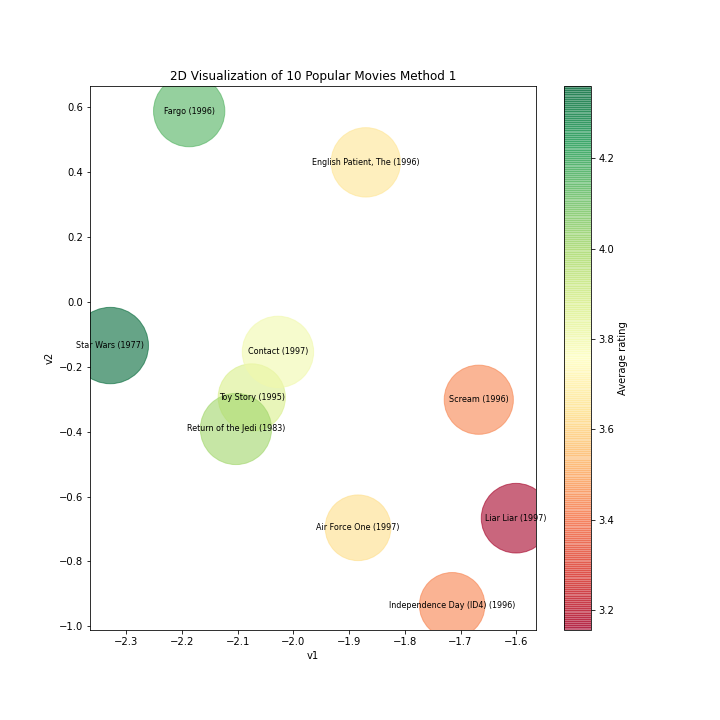
\includegraphics[width=0.5\textwidth]{matrixfactorization/2D Visualization of 10 Popular Movies Method 1.png}
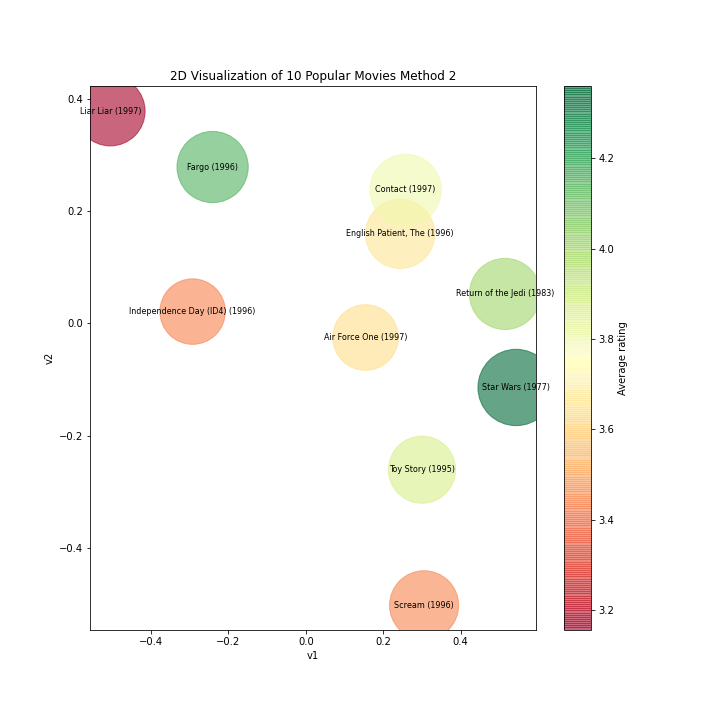
\includegraphics[width=0.5\textwidth]{matrixfactorization/2D Visualization of 10 Popular Movies Method 2.png}
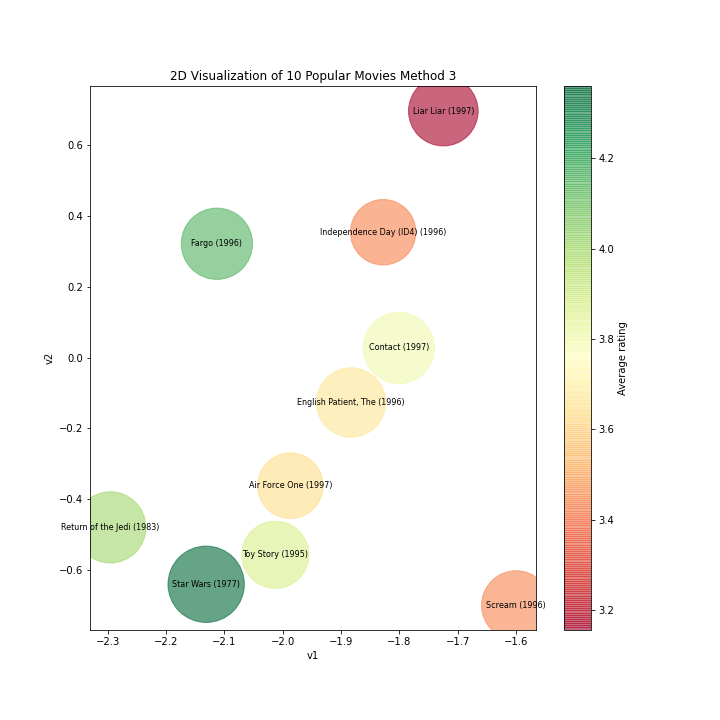
\includegraphics[width=0.5\textwidth]{matrixfactorization/2D Visualization of 10 Popular Movies Method 3.png}
\end{figure}

\newpage

\subsection{10 Best Movies}

\begin{figure}[H]
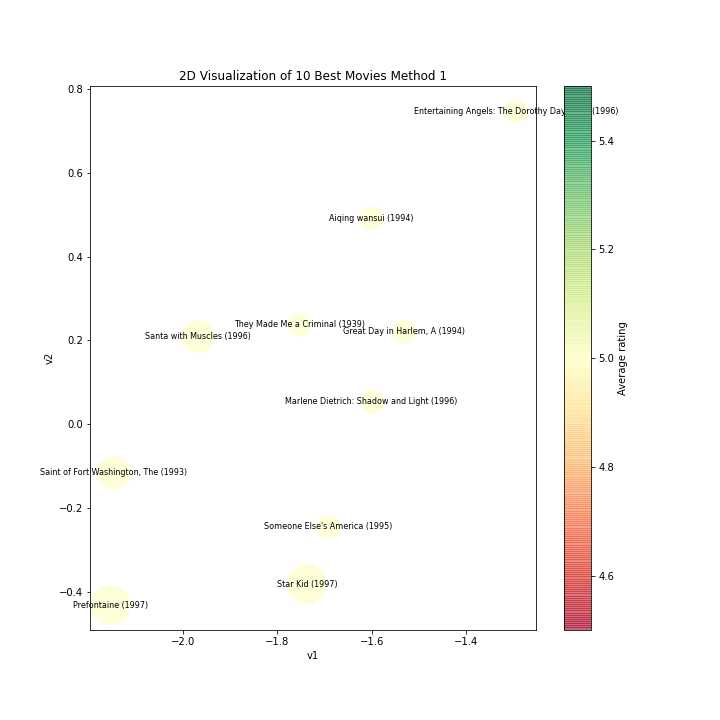
\includegraphics[width=0.5\textwidth]{matrixfactorization/2D Visualization of 10 Best Movies Method 1.png}
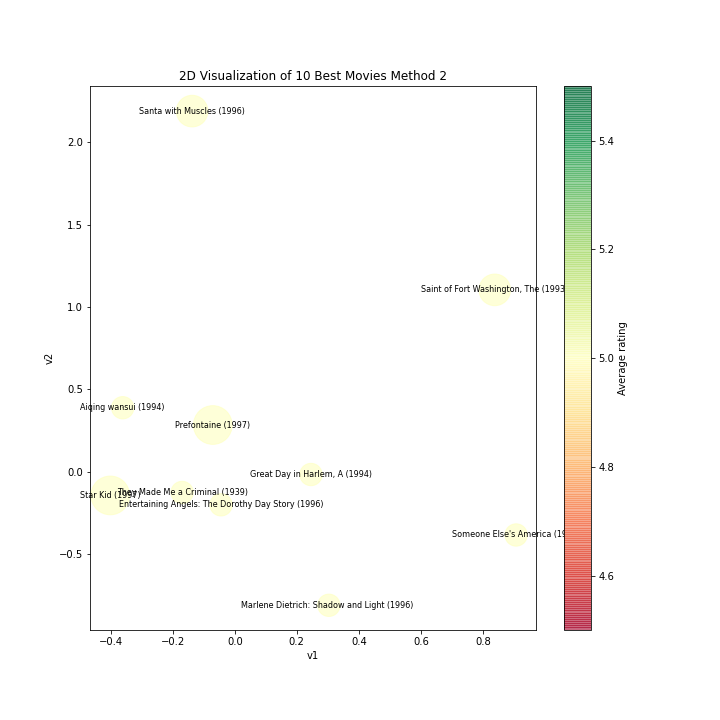
\includegraphics[width=0.5\textwidth]{matrixfactorization/2D Visualization of 10 Best Movies Method 2.png}
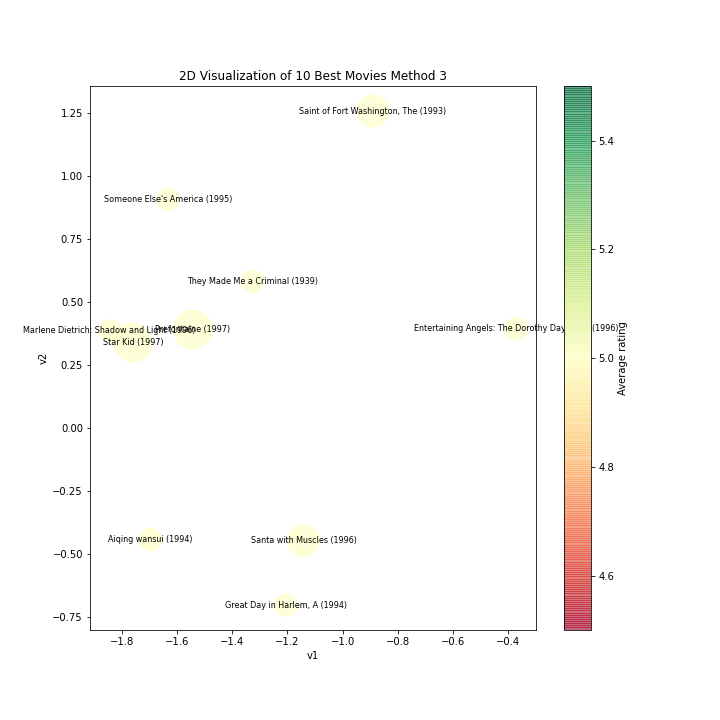
\includegraphics[width=0.5\textwidth]{matrixfactorization/2D Visualization of 10 Best Movies Method 3.png}
\end{figure}

\newpage


\subsection{10 Movies from Three Genres Selected}


\paragraph{Action Above}
\begin{figure}[H]
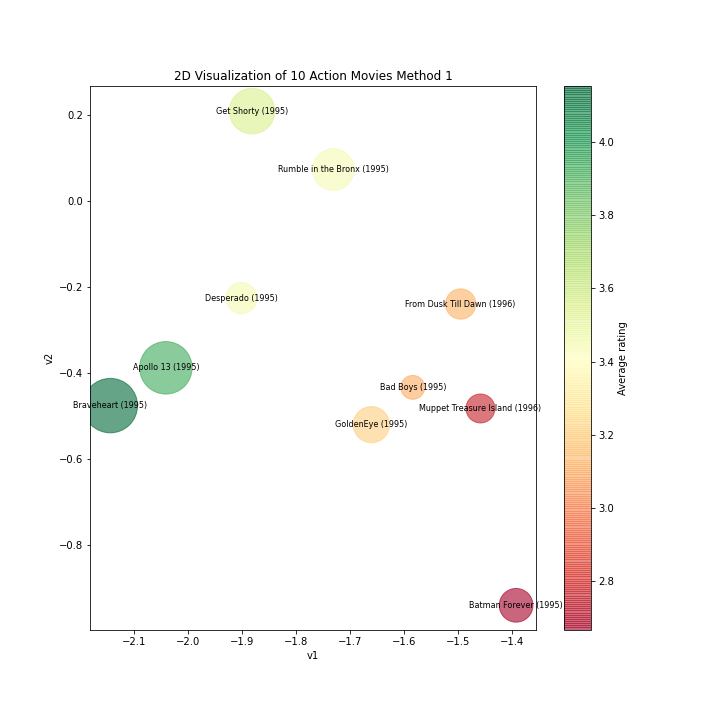
\includegraphics[width=0.5\textwidth]{matrixfactorization/2D Visualization of 10 Action Movies Method 1.png}
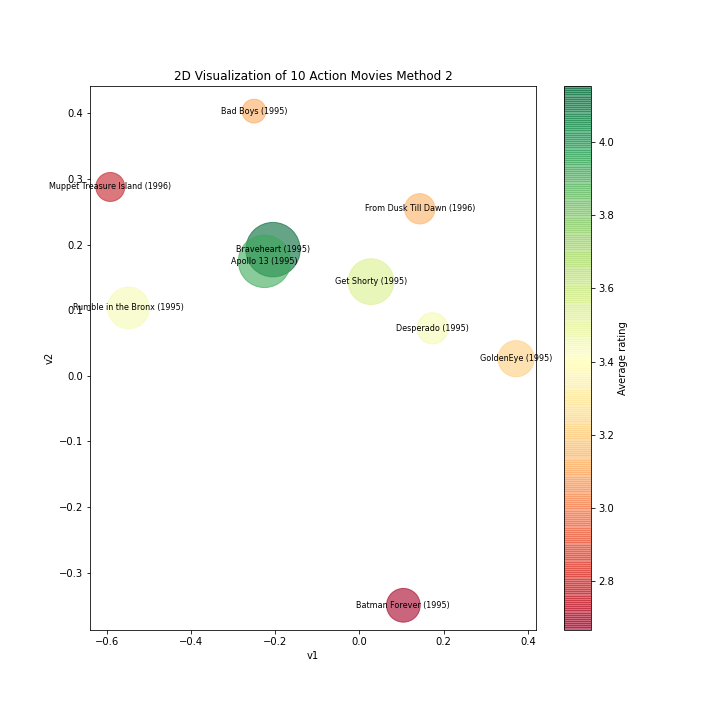
\includegraphics[width=0.5\textwidth]{matrixfactorization/2D Visualization of 10 Action Movies Method 2.png}
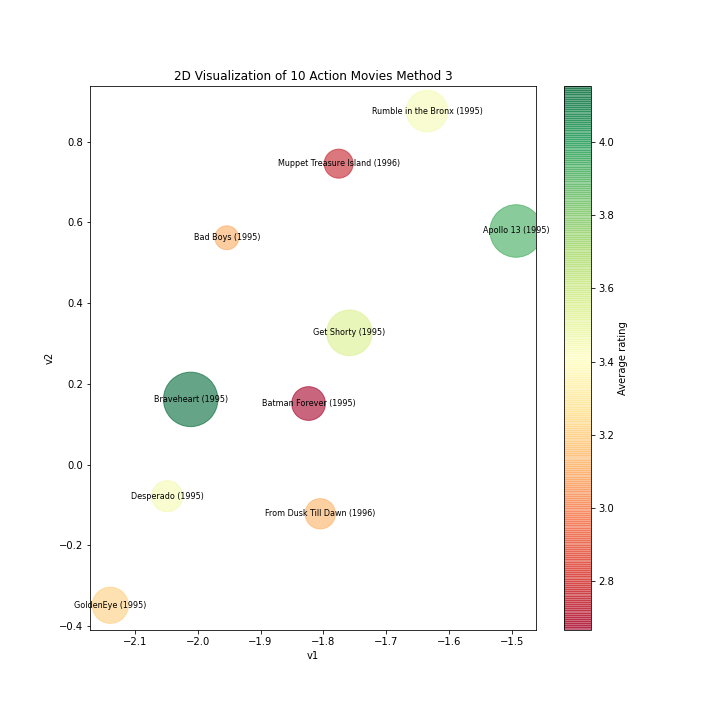
\includegraphics[width=0.5\textwidth]{matrixfactorization/2D Visualization of 10 Action Movies Method 3.png}
\end{figure}

\newpage

\paragraph{Horror Above}

\begin{figure}[H]
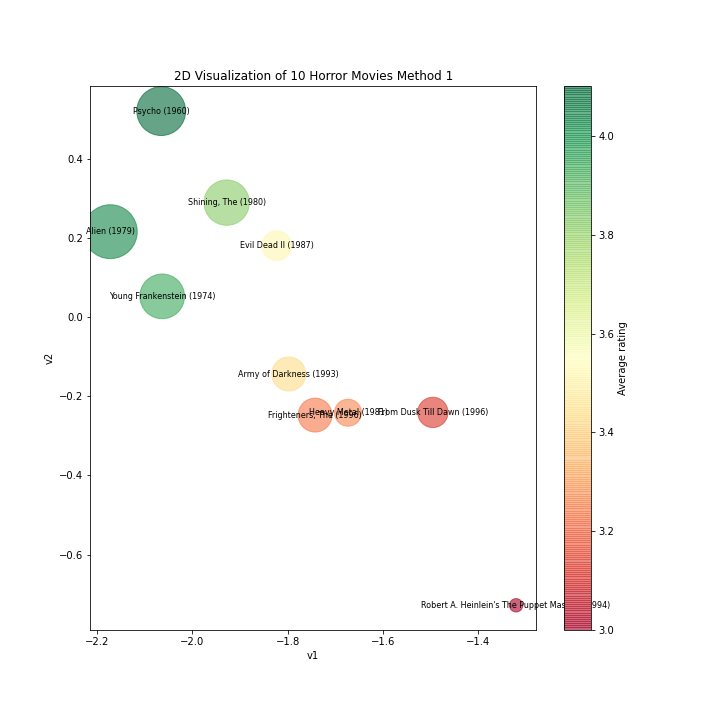
\includegraphics[width=0.5\textwidth]{matrixfactorization/2D Visualization of 10 Horror Movies Method 1.png}
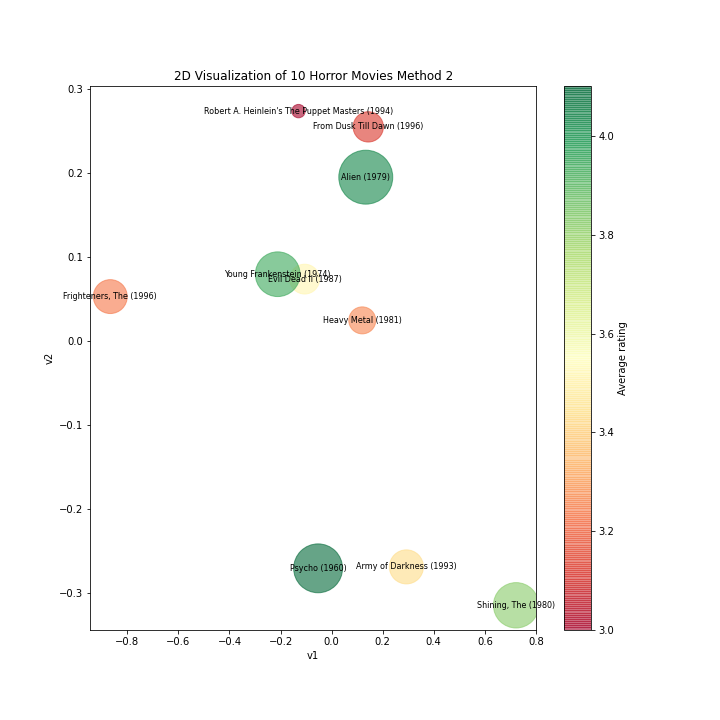
\includegraphics[width=0.5\textwidth]{matrixfactorization/2D Visualization of 10 Horror Movies Method 2.png}
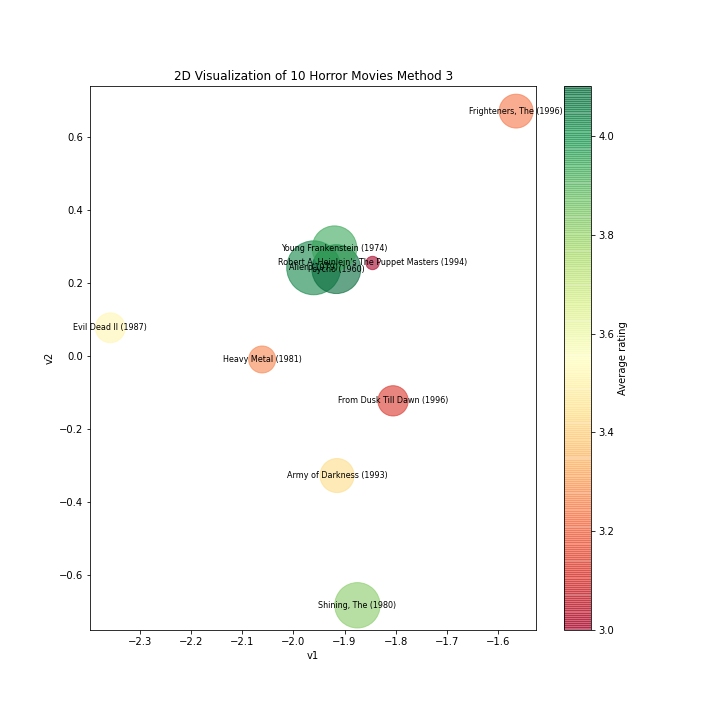
\includegraphics[width=0.5\textwidth]{matrixfactorization/2D Visualization of 10 Horror Movies Method 3.png}
\end{figure}

\newpage

\paragraph{Comedy Above}

\begin{figure}[H]
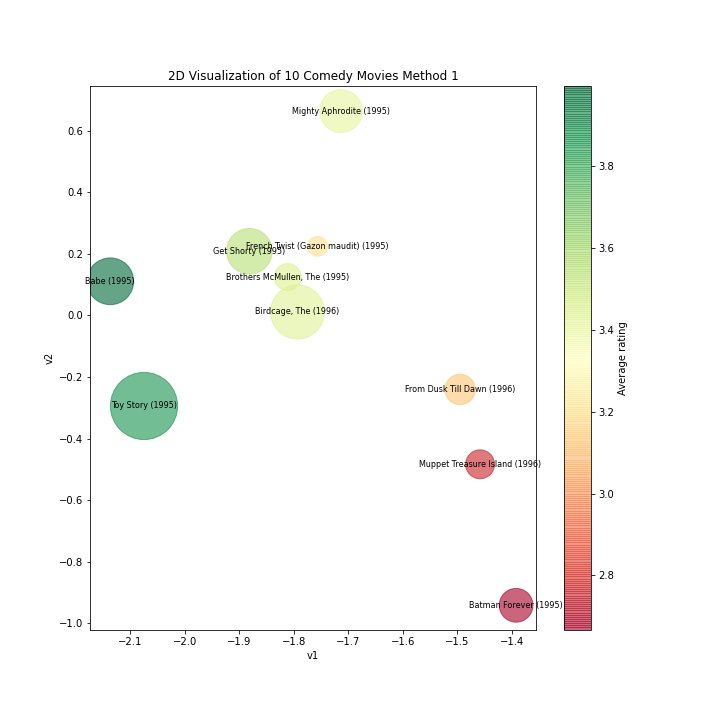
\includegraphics[width=0.5\textwidth]{matrixfactorization/2D Visualization of 10 Comedy Movies Method 1.png}
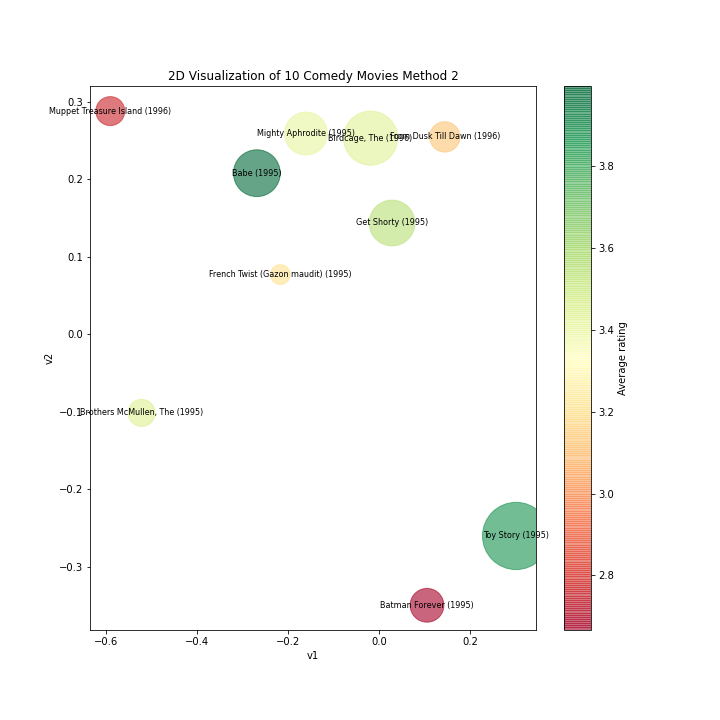
\includegraphics[width=0.5\textwidth]{matrixfactorization/2D Visualization of 10 Comedy Movies Method 2.png}
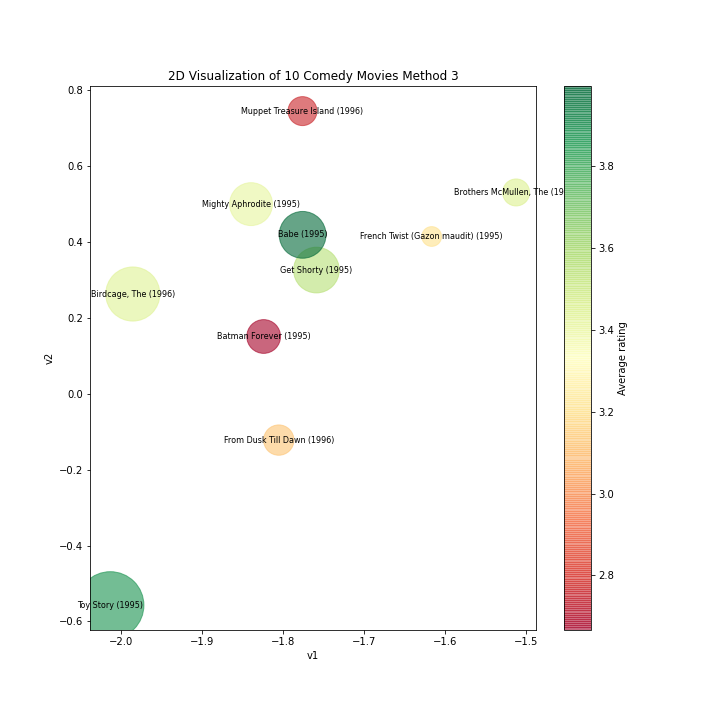
\includegraphics[width=0.5\textwidth]{matrixfactorization/2D Visualization of 10 Comedy Movies Method 3.png}
\end{figure}

\newpage

It can be observed that movies that that are similar in nature are classified in similar regions in the visualization. For example, in our action movie classification, the movies Apollo 13 and Braveheart are visualized to be very similar, which makes sense since they are similar movies. This matches what we expect to see, since these movies are similar and are closely place in the visualization. There is not any clear pattern between the visualization of the best movies and the visualization of the popular movies. However, for the best movies, there is a smaller pool of ratings, while for the most popular movies there is a variety of ratings. Amongst the genres chosen, generally the movies with the highest average rating are grouped together. This leads us to believe that in any specific category, there are usually only a few types or general patterns of movies that lead to higher ratings. This is especially shown in the horror category:
\begin{figure}[H]
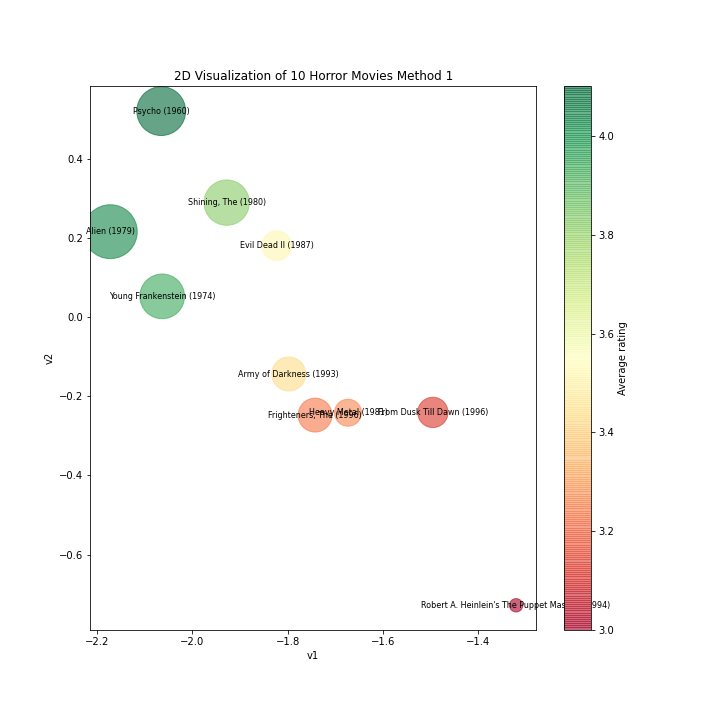
\includegraphics[width=0.5\textwidth]{matrixfactorization/2D Visualization of 10 Horror Movies Method 1.png}
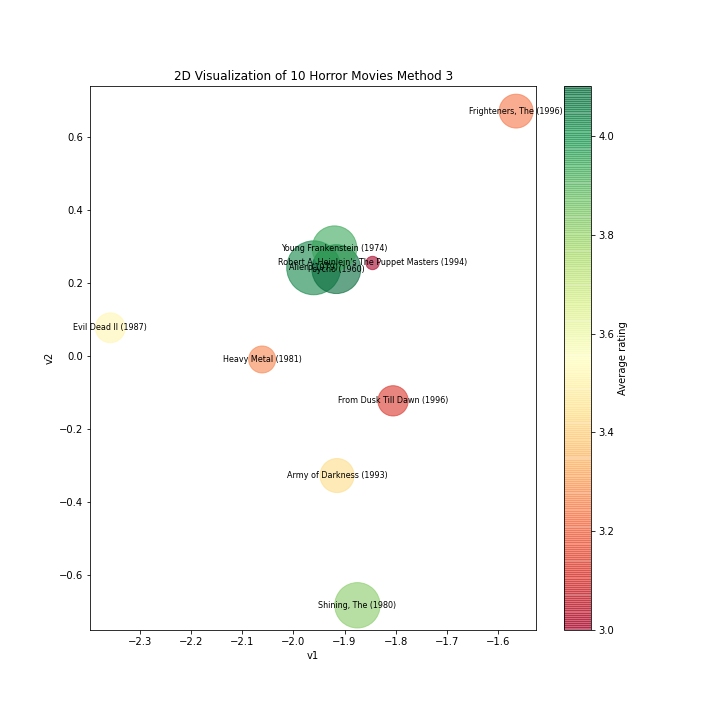
\includegraphics[width=0.5\textwidth]{matrixfactorization/2D Visualization of 10 Horror Movies Method 3.png}
\end{figure}
\end{document}

